

The processes we are interested in looking at in this thesis involve superpartners of leptons, gauge bosons, and the Higgs boson. Besides this, we will look at a dark matter particle candidate, which is predicted to be the lightest supersymmetric particle (LSP).  This thesis looks at proton-proton collisions with final state two leptons and missing transverse energy (MET/$E_T^{miss}$). The SUSY processes we are looking at are direct slepton production, chargino production with slepton/sneutrino-mediated-decays and with W-boson-mediated-decays. 


In figure \ref{fig:SlepSlepFeynman} below, we can see the direct slepton production as a production of two hypothetical sleptons which decay to the final state, comprising of two leptons and missing transverse energy (i.e. missing energy in the detector). The neutralinos, which are the MET in this process, are a mixture of the sparticles photino, zino, and higgsino and is also one of the dark matter candidates mentioned above.  
\begin{figure}[H]
    \centering
    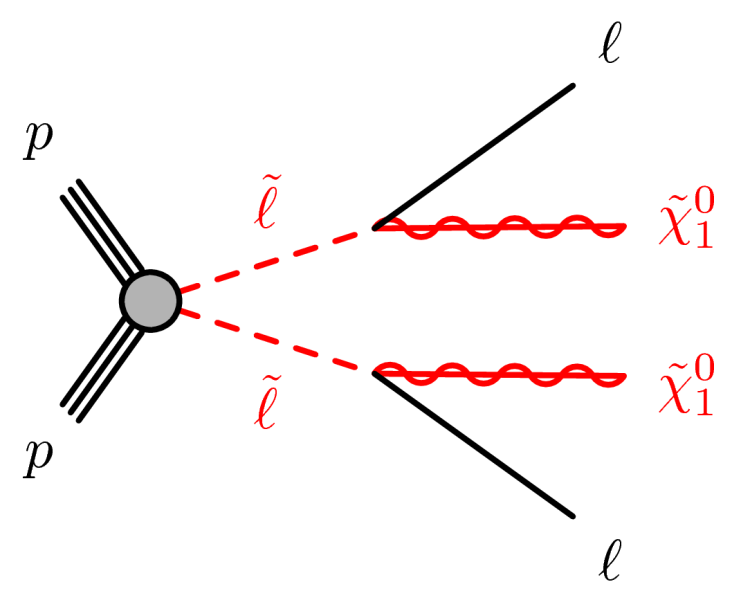
\includegraphics[width = 0.4\textwidth]{Figures/FeynmanDiagrams/SlepSlepFeynman.png}
    \caption{Direct slepton production $pp \rightarrow \tilde{l}^+ \tilde{l}^- \rightarrow l^+l^- + \tilde{\chi}_1^0 \tilde{\chi}_1^0$.}
    \label{fig:SlepSlepFeynman}
\end{figure}

In figure \ref{fig:SlepSnuFeynman} and \ref{fig:WWFeynman} we can see the chargino production with  slepton/sneutrino-mediated-decays and with W-boson-mediated-decays. Charginos are a mixture of the sparticles wino and the charged higgsino. These processes have the same final state as direct slepton production, but here the neutrinos are also a part of the MET, since we can't actually detect them in the detector. 
\begin{figure}[H]
    \centering
    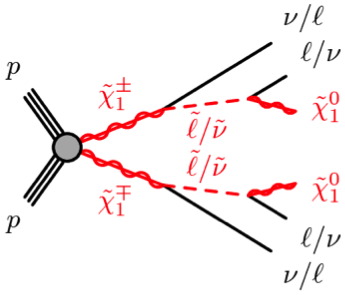
\includegraphics[width = 0.4\textwidth]{Figures/FeynmanDiagrams/SlepSnuFeynman.png}
    \caption{Chargino production with slepton/sneutrino-mediated-decays $pp \rightarrow \tilde{\chi}_1^+ \tilde{\chi}_1^- \rightarrow \tilde{l}^+ \tilde{l}^- /\tilde{\nu} \tilde{\nu} \rightarrow l^+l^- + \nu \Bar{\nu} + \tilde{\chi}_1^0 \tilde{\chi}_1^0$.}
    \label{fig:SlepSnuFeynman}
\end{figure}

\begin{figure}[H]
    \centering
    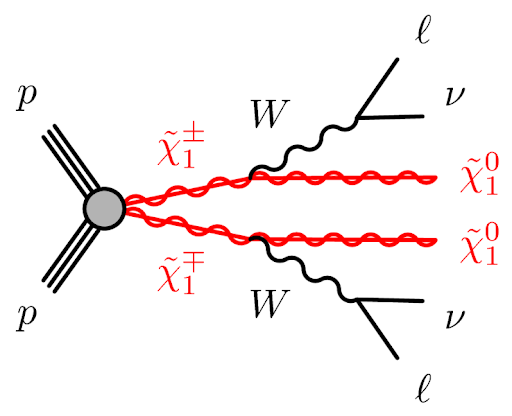
\includegraphics[width = 0.4\textwidth]{Figures/FeynmanDiagrams/WWFeynman.png}
    \caption{Chargino production with W-boson-mediated-decays $pp \rightarrow \tilde{\chi}_1^+ \tilde{\chi}_1^- \rightarrow W^+ W^- \rightarrow l^+l^- + \nu \Bar{\nu} + \tilde{\chi}_1^0 \tilde{\chi}_1^0$.}
    \label{fig:WWFeynman}
\end{figure}

The DM process we are looking at in this thesis is the mono-Z process shown in figure \ref{fig:monoZFeynman2}. Here we have a mediator V which decays into the DM particles $\chi$ and a W/Z that decays into two leptons. This gives us the same final state as we had for the SUSY processes.  

\begin{figure}[H]
    \centering
    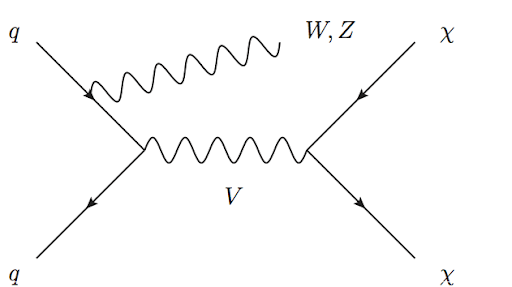
\includegraphics[width = 0.4\textwidth]{Figures/FeynmanDiagrams/monoZFeynman2.png}
    \caption{Mono-Z process $pp \rightarrow Z + MET \rightarrow l^+ l^- + MET$.}
    \label{fig:monoZFeynman2}
\end{figure}


\section{MC simulated events}

The data taken into consideration is from the ATLAS experiment at LHC between 2015-2018 (Run 2), further explained in chapter \ref{sec:LHCandATLAS}. But, we are also looking at some MC simulated background and signal which will be explained in this section. The explanations are taken from the publications from ATLAS, namely \cite{sleptonexclusion} for the SUSY signals and \cite{monoZexclusion} for the mono-Z signal. We present an overview of what signal samples that are used in table \ref{tab:directslepLOW} - \ref{tab:MonoZHigh} in section \ref{sec:sigsamptab}. 

The SUSY signal samples were generated from leading-order (LO) matrix elements with up to two extra partons using \textsc{MadGraph5\_aMC@NLO 2.6.1} \cite{48} interfaced to \textsc{Pythia 8.186} \cite{49}, with the A14 tune \cite{50}, for the modelling of the SUSY decay chain, parton showering, hadronisation and the description of the underlying event. Parton luminosities were provided by the NNPDF2.3LO PDF set \cite{51}. Jet–parton matching was performed following the CKKW-L prescription \cite{52}, with a matching scale set to one quarter of the mass of the pair-produced SUSY particles. Signal cross-sections were calculated to next-to-leading order (NLO) in $\alpha_s$ adding the resummation of soft gluon emission at next-to-leading-logarithm accuracy(NLO+NLL) \cite{53,54,55,56,57,58,59}. The nominal cross-sections and their uncertainties were taken from an envelope of cross-section predictions using different PDF sets and factorisation and renormalisation scales, as described in Ref. \cite{60}. 


To study the invisible Higgs boson decays, Monte Carlo events are produced for the SM ZH process with a subsequent Z boson decay into a dilepton pair and the H$\rightarrow$ZZ$\rightarrow \nu \nu \nu \nu$ decay (ZH$\rightarrow ll$+inv). The ZH signal processes from both the quark–antiquark (qqZH) and gluon–gluon (ggZH) initial states are modelled with \textsc{Powheg-Box v2} \cite{49Z, 50Z} using the CT10 \cite{51Z} parton distribution function (PDF) and interfaced to \textsc{Pythia8.186} \cite{52Z} for parton showering. The kinematic distributions of ZH$\rightarrow ll$ +inv events are described at next-to-leading-order (NLO) in QCD. Additionally, for the qqZH process, the MINLO \cite{53Z} method is applied to improve the gluon resummation calculation, and the $p_T^Z$ distribution is corrected to NLO electroweak (EW) accuracy with a reweighting approach detailed in Ref. \cite{3Z}. The SM ZH production cross-section is computed with next-to-next-to-leading-order (NNLO) QCD and NLO EW precision and found to be 884 fb \cite{3Z} with $m_H = 125$ GeV at 13 TeV. The DM signal is modelled with the leading-order \textsc{MadGraph5\_aMC@NLO} matrix element \cite{54Z} using NNPDF3.0 \cite{55Z} and showered with Pythia8.186. DM signal events with an axial-vector mediator and fermionic WIMPs are produced for different $m_{med}$ and $m_\chi$, both in a range from 10 to 1000 GeV.  As recommended in Ref. \cite{44Z}, the DM events are generated by choosing $g_q = 0.25$, $g_\chi = 1$, and a minimal mediator width. The AZNLO \cite{56Z} and A14 \cite{57Z} parameter sets are used to tune the \textsc{Pythia8.186} parton-shower for the simulation of the ZH $\rightarrow ll$+inv and DM signals, respectively.


The different backgrounds that we are considering are diboson, triboson, $t\Bar{t}$, single top, other top events ($t\Bar{t}$ events with a pair of leptons or boson(s)), Higgs, Drell-Yan, Z+jets and W+jets. The MC samples are simulated using different generators that are listed up in table \ref{tab:bkg_samples}. The goal is to separate these backgrounds from the signals we are looking at, which consist in the four different processes that we looked at earlier in this chapter. 

\begin{table}[H]
    \centering
    \begin{tabular}{l l l l} \toprule
        \textbf{Background sample} & \textbf{Generator} & \textbf{Parton shower} & \textbf{Normalisation}\\
        \midrule
        \midrule
        Diboson & \textsc{Sherpa2.2.2}\cite{sherpa2_1, sherpa1_2, sherpa1_3} & \textsc{Sherpa2.2.2} & NLO \cite{NLO}\\
        Triboson & \textsc{Sherpa2.2.2} & \textsc{Sherpa2.2.2} & NLO \\
        Z+jets & \textsc{Sherpa2.2.1} \cite{sherpa1_1, sherpa1_2, sherpa1_3} & \textsc{Sherpa2.2.1} & NNLO \cite{NNLO}\\
        W+jets & \textsc{Powheg-Box v2}\cite{49Z, 50Z} & \textsc{Pythia8.186} \cite{49} & NLO\\
        Drell-Yan & \textsc{Sherpa2.2.1} & \textsc{Sherpa2.2.1} & NNLO\\
        $t\Bar{t}$ & \textsc{Powheg-Box v2} & \textsc{Pythia8.186} & NNLO\\
        Single top & \textsc{Powheg-Box v2} & \textsc{Pythia8.186} & NLO\\
        topOther & \textsc{MG5\_aMC@NLO} \cite{48} & \textsc{Pythia8.186} & NLO\\
        Higgs & \textsc{Powheg-Box v2} & \textsc{Pyhtia8.186} & NLO\\
        \bottomrule
    \end{tabular}
    \caption{An overview of the different generators used to simulate the MC background samples.}
    \label{tab:bkg_samples}
\end{table}


Before we move on to how we perform the analysis, we also need to know how we are going to know that we see SUSY and DM particles in the detector. Since they never have been discovered, we have to lean on some hypotheses on how this is happening. As for all events in the detector, we have to reconstruct the events using their decays. The supersymmetric particles are expected to decay into cascades that will contain a LSP which will interact very weakly with the detector material which again will result in a big measured MET in the detector. The rest of the cascade will result in a final state with with leptons and/or jets. Together with the MET this gives us the final state we are looking for. For the mono-Z process we can measure the MET from the DM particles decayed from the unknown hypothetical mediator particle. Together with the leptons we get from the decay of the Z-boson, this gives us the same final state as for the SUSY processes.




































\begin{comment}

\begin{itemize}
    \item Bruker noe som eksisterer
    \item Tradisjonell måte ting har blitt gjort på
    \item begrenset av menneskets forståelse av prosessen vi ser på
    \item vi må bestemme alle kuttene som blir gjort
    \item Du må vite hva du skal se etter for å gjøre dette, altså trenger en teori/hypotese
    \item Tenk overgang til ML
    \item Valg må være begrunnet 
    \item Massesplitting. Cut and count er svak på lav massesplitting. Dette gjør ML bedre
\end{itemize}
\end{comment}





